\section{Implementación}
La implementación del programa se realizó mediante el lenguaje de programación C. Las funciones necesarias fueron implementadas en archivos separados según su funcionalidad. El código puede ser compilado directamente mediante un \texttt{Makefile}, el cual se encuentra en el directorio raíz.

\subsection{Estructura de directorios}
Dentro del directorio \texttt{src} se encuentran los siguientes archivos:

\begin{itemize}
    \item \texttt{errors.c}: Contiene las funciones de gestión de errores.
    \item \texttt{files.c}: Contiene las funciones de gestión de archivos.
    \item \texttt{graph.c}: Contiene las funciones de gestión del grafo.
    \item \texttt{hash.c}: Contiene las funciones de hashing.
    \item \texttt{link\_list.c:} Contiene las funciones de gestión de listas enlazadas.
    \item \texttt{main.c}: Contiene el código principal del programa.
    \item \texttt{page\_rank.c}: Contiene lo necesario para el cálculo del PageRank.
    \item \texttt{reverse\_index.c}: Contiene las funciones de gestión del índice invertido.
    \item \texttt{stop\_words.c}: Contiene las funciones de gestión de stop words.
    \item \texttt{timer.c}: Contiene las funciones de gestión del temporizador.
    \item \texttt{utilities.c}: Contiene funciones generales.
\end{itemize}

Por otro lado, en la carpeta \texttt{testing} se encuentran archivos para realizar pruebas del programa:
\begin{itemize}
    \item \texttt{spanish.txt}: Contiene una lista de stopWords\footnote{Una StopWord es un tipo de palabra muy común en un idioma, en este caso en Español. Estas no deberían de ser consideradas para su almacenamiento en el indice invertido dada su recurrencia y la poca información entregada por su aparición en un documento.} en español extraídas de la referencia \cite{SpanishStopWords}; estas se tienen en cuenta a la hora de procesar los archivos así como a la hora de buscar palabras clave.
    \item \texttt{doc\_generator.py}: Script de \textit{Python} que recupera de \textit{Wikipedia} artículos aleatorios con el fin de capturar archivos de prueba ``realistas'' para el programa.
\end{itemize}

\subsection{Estructuras de datos}

\subsubsection{Manejo de archivos}
Para el manejo de archivos se optó por utilizar una \textit{lista enlazada simple} para almacenar los archivos, en la cual cada uno de ellos se guarda en un bloque de la lista. Esto permite una búsqueda más eficiente y sin un límite de memoria. Además, para poder identificar y procesar los archivos del directorio y sus sub-directorios se utilizó la librería \texttt{Dirent.h} \cite{Dirent.h}.

La librería \texttt{dirent.h} es una librería de C que permite leer los archivos de un directorio, y que proporciona una estructura llamada \textit{struct dirent} que contiene información sobre cada archivo, como por ejemplo su nombre (con extensión), su tipo (archivo regular o directorio) y su identificador (ID). También se utiliza la estructura \textit{DIR} para manejar el directorio abierto.

En el caso de existir un sub-directorio dentro del directorio de entrada, se procesará recursivamente, añadiendo cada archivo que se encuentre en dicho sub-directorio a la lista de archivos.

Por último para identificar los archivos que contienen texto plano, se utilizó la función \texttt{is\_valid\_extension()} para extraer el nombre sin extensión y a su vez verificar si el archivo es de texto plano a traves de su extensión.

\subsubsection{Índice invertido} \label{subsec:ImplIndiceInvertido}
Para el índice invertido se optó finalmente por utilizar una \textit{tabla hash} para almacenar las palabras, permitiendo así una búsqueda eficiente. Sin embargo, surge la necesidad de manejar posibles colisiones y el límite de memoria que trae consigo los arreglos. Para solucionar esto, se optó que cada celda de esta tabla hash contenga una \textit{lista enlazada simple}, donde realmente se almacenarán las palabras asociadas a un hash key. Esto permite una búsqueda más eficiente y sin un límite de memoria (más que el de la propia máquina).

Por otro lado, para poder relacionar un archivo con una palabra se hizo que cada una de ellas almacene consigo otra \textit{lista enlazada simple}, en la cual se almacenarán punteros a los archivos que contienen dicha palabra, además de guardar información sobre los párrafos en los que aparece dicha palabra (manejados con otra LES adicional).

Para comprender mejor la estructura de datos de este índice invertido, se presentará la figura \ref{fig:reverse_index}.

\begin{figure}[h!]
    \centering
    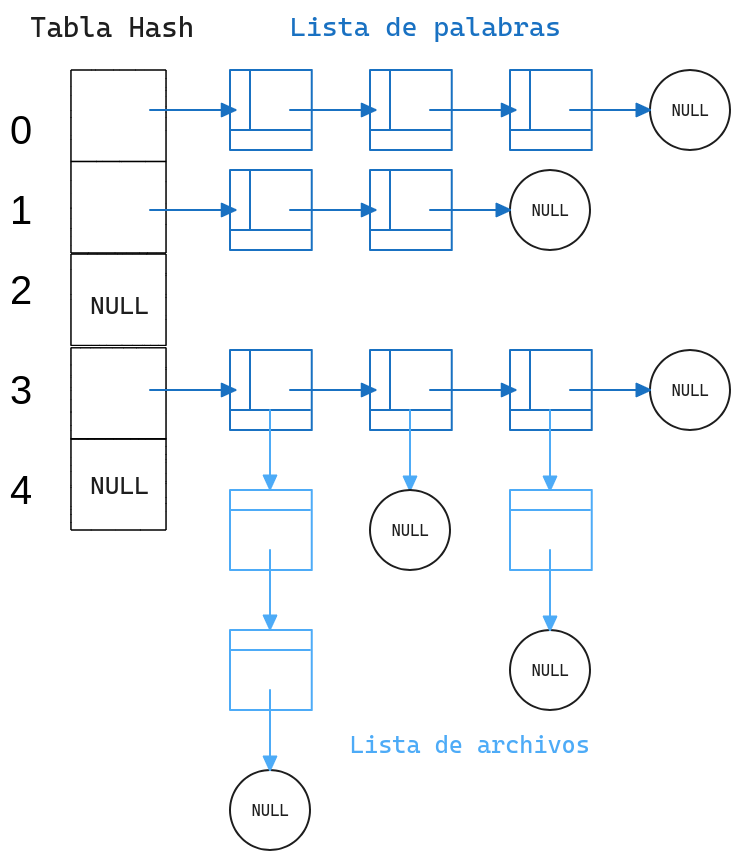
\includegraphics[width=0.5\textwidth]{src/figures/reverse_index.png}
    \caption{Esquema de la estructura de datos del índice invertido}
    \label{fig:reverse_index}
\end{figure}

Debido a que el uso de \textit{listas enlazadas simples} esta ligado a una busqueda secuencial, como una manera de mitigar la ineficiencia de esto, se implemento la funcion \texttt{move\_to\_front()}, la cual mueve un nodo al principio de la lista. Entonces, cuando un nodo es buscado, éste queda al principio de la lista, así las palabras más buscadas por el usuario pueden volver a buscarse en menos tiempo.


\subsubsection{Grafos}
\label{subsec:ImplGrafos}
La implementación del grafo de archivos es muy similar a la del índice invertido (un Esquema similar al observado en la figura \ref{fig:reverse_index}):
\begin{itemize}
    \item Un arreglo de tamaño fijo conteniendo las keys de la tabla hash.
    \item Una lista para cada elemento del arreglo, conteniendo los nodos asociados a dicha key.
    \item Dentro de cada nodo se almacena información del archivo al que hace referencia (Puntero a la estructura de datos para el almacenamiento de los archivos) así como una lista de enlaces adyacentes e incidentes.
\end{itemize}

El uso de Tablas Hash para esta solución permite una gran eficiencia de lectura-escritura, dando también espacio a un correcto manejo de memoria dinámica.

Cabe destacar que el grafo implementado es un \textit{Grafo Dirigido} lo cual quiere decir que un enlace del nodo $n_1$ al $n_2$ es diferente al enlace desde $n_2$ a $n_1$ (lo que tiene sentido si se piensa en el comportamiento de los enlaces en un sistema de archivos).

\subsection{PageRank}
En el caso del \textit{PageRank}, su implementación se realizo mediante la adaptación de la formula de PageRank (\ref{eq:PageRank}) a un grafo dirigido (como se explicó en la sección \ref{subsec:ImplGrafos}). Para la construcción de la función \texttt{calculate\_page\_rank()} se utilizó la estructura de datos \textit{Graph}, de la cual se obtuvieron los nodos y las listas de adyacencias e incidencia de estos.

Con el fin de ser consecuentes con lo planteado en \ref{Subsec:PageRank}, se tomó la cantidad total de nodos como el total de archivos en el directorio, y se asigno un valor inicial de $\frac{1}{N}$ a cada uno de los nodos, donde $N$ es la cantidad total de nodos. Luego, se realizan las iteraciones necesarias para la convergencia del algoritmo, en el cual se actualiza el valor de cada nodo con la formula de PageRank (\ref{eq:PageRank}), y se calcula el error de la iteración. Si el error es menor a un valor de frontera, se detiene el algoritmo y se retorna el valor de PageRank de cada nodo.

Es importante resaltar que el valor de frontera utilizado corresponde a $1 \times 10^{-4}$, el cual fue seleccionado de manera arbitraria. Y el valor de damping factor utilizado fue de $0.85$, el cual es el valor estándar a la hora de implementar el PageRank.

\subsection{implementaciones extra}
\subsubsection*{Temporizador}
Se implementó un temporizador utilizando la librería \texttt{time.h} para medir los tiempos de ejecución de las funciones, para analizar y mejorar el código (sólo para uso interno).

\subsubsection*{MergeSort}
Se utilizó \textit{MergeSort} para ordenar (de mayor a menor) los archivos en los que aparece cada palabra según el PageRank de los nodos que referencian, para tener una correcta visualización de los resultados.

Se decidió optar por este algoritmo de ordenamiento, dada su eficiencia sobre otros algoritmos tales como el \texttt{InsertionSort} o el \texttt{SelectionSort}.

\subsubsection*{Interacción con el usuario}

En cuanto a la interacción con el usuario, se llevó a cabo una impresión por pantalla del procesamiento de los diversos archivos, para luego solicitar al usuario la palabra que desea buscar. Una vez ingresada una palabra se muestran los archivos con coincidencias y se le solicita al usuario que seleccione un archivo para mostrar el contenido del mismo. Para esta última tarea se implemento la función \texttt{print\_file\_paragraphs()} la cual imprime por pantalla los párrafos del archivo seleccionado en donde se encuentra la palabra.

Para la realización de esto se obtuvo el byte de inicio de cada uno de los párrafos en los que se encuentra cada palabra al ser ingresada a la tabla de indice invertido \ref{subsec:ImplIndiceInvertido}, mediante la función \texttt{process\_files()}.